\begingroup
\renewcommand{\arraystretch}{0}
\setlength{\tabcolsep}{0pt}
\begin{figure}[bth]
\centering
\begin{tabular}{l|cc|cc|cc} 
\parbox[t]{4mm}{\multirow{3}{*}{\rotatebox[origin=c]{90}{Mass Imbalance}}}&
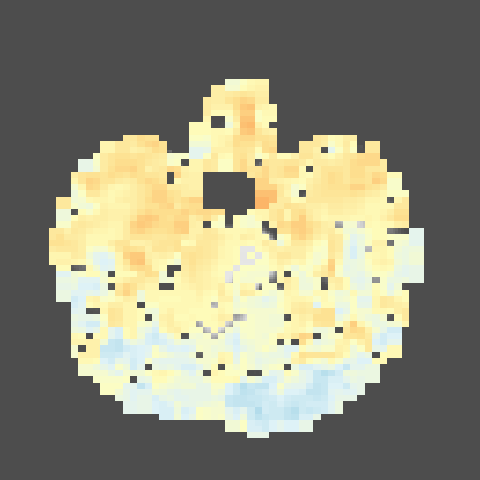
\includegraphics[width=0.16\linewidth]{cor-axial-age-mW} &
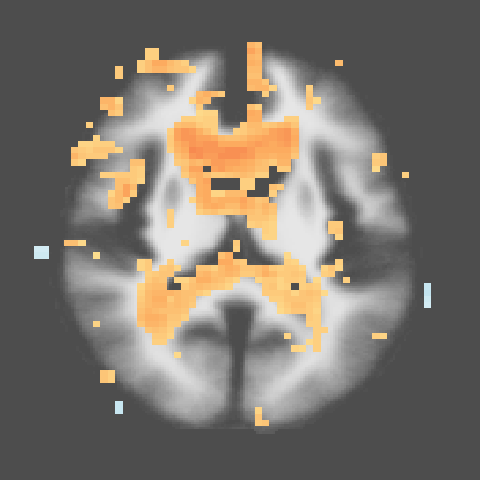
\includegraphics[width=0.16\linewidth]{cor-axial-age-t-mW} &
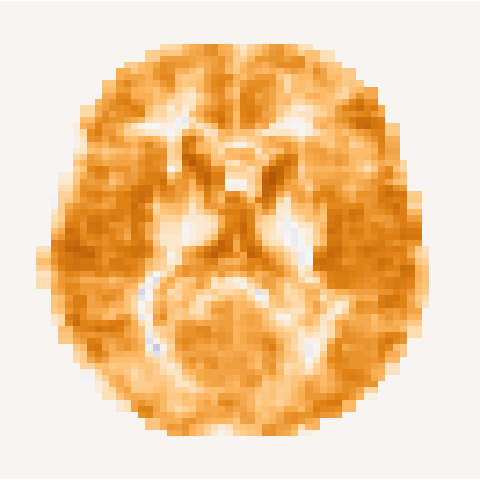
\includegraphics[width=0.16\linewidth]{cor-axial-cdr-mW} &
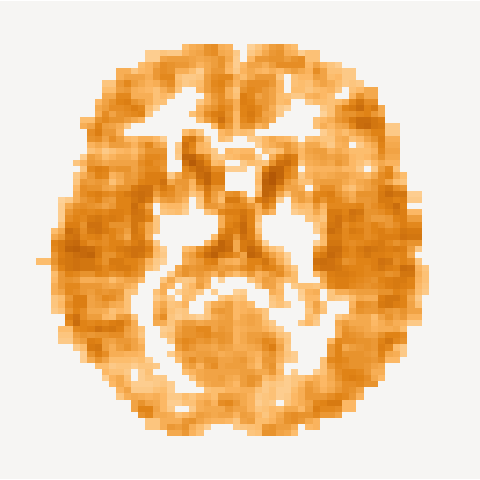
\includegraphics[width=0.16\linewidth]{cor-axial-cdr-t-mW} &
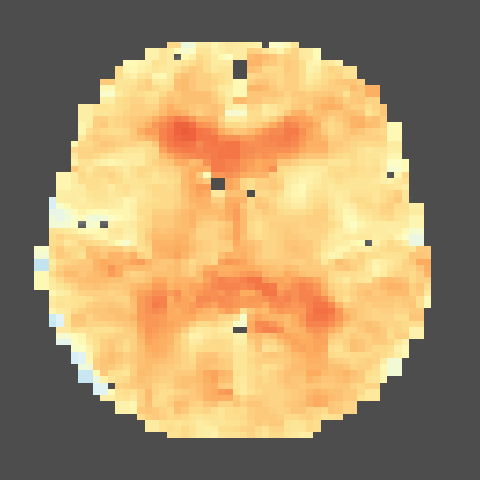
\includegraphics[width=0.16\linewidth]{cor-axial-mmse-mW} &

\includegraphics[width=0.16\linewidth]{cor-axial-mmse-t-mW} \\ 
%
        &
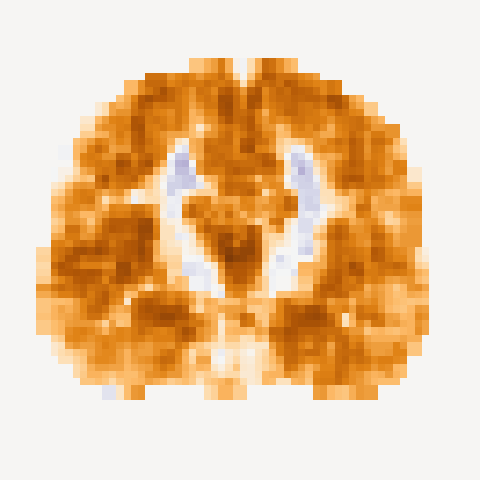
\includegraphics[width=0.16\linewidth]{cor-coronal-age-mW} &
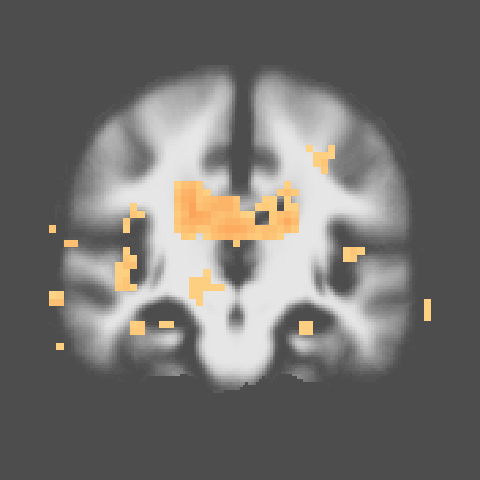
\includegraphics[width=0.16\linewidth]{cor-coronal-age-t-mW} &
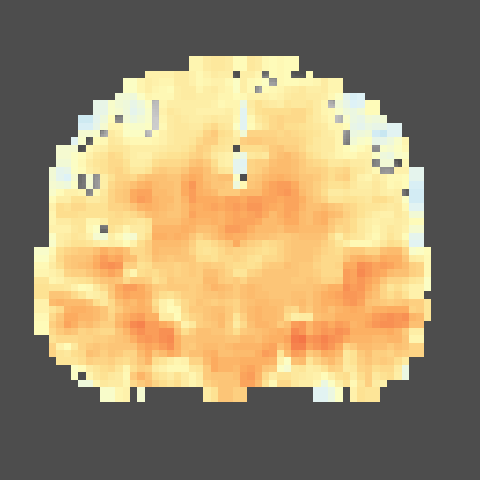
\includegraphics[width=0.16\linewidth]{cor-coronal-cdr-mW} &
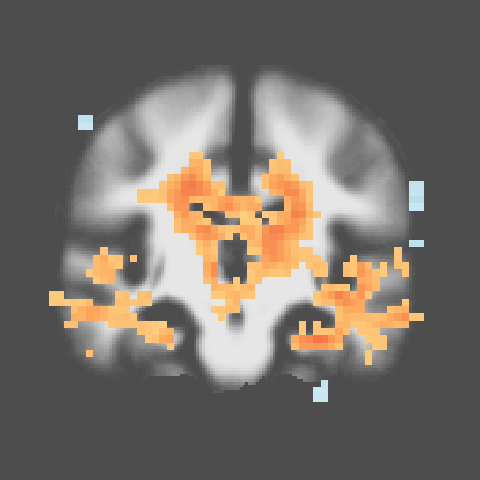
\includegraphics[width=0.16\linewidth]{cor-coronal-cdr-t-mW} &
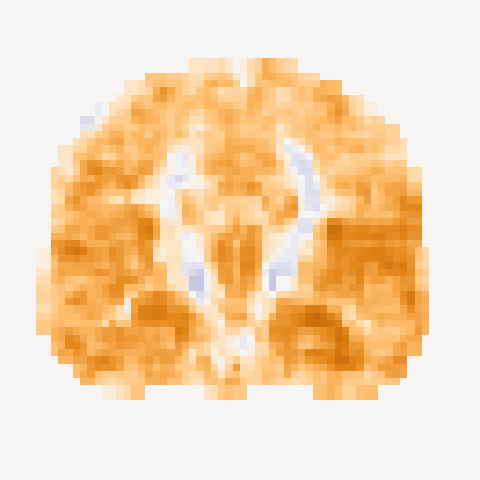
\includegraphics[width=0.16\linewidth]{cor-coronal-mmse-mW} &
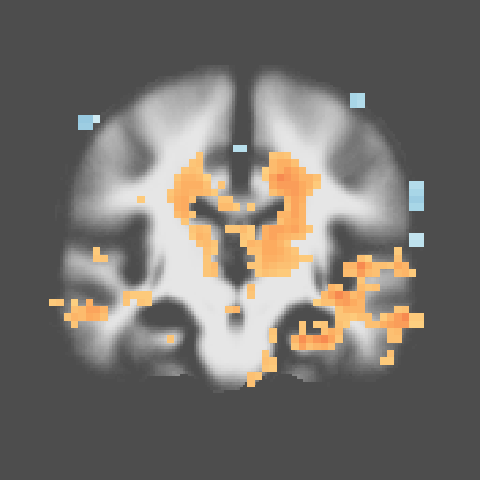
\includegraphics[width=0.16\linewidth]{cor-coronal-mmse-t-mW} \\ 
%
        &
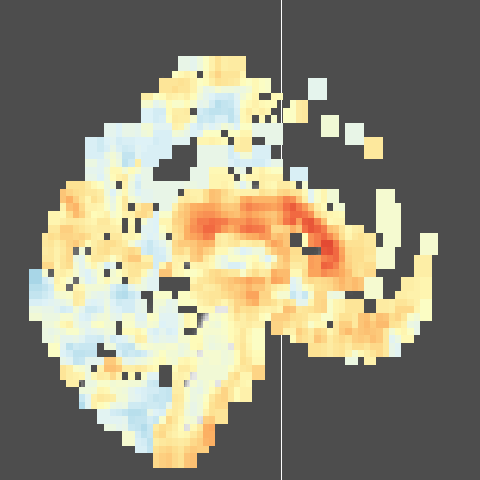
\includegraphics[width=0.16\linewidth]{cor-sagital-age-mW} &
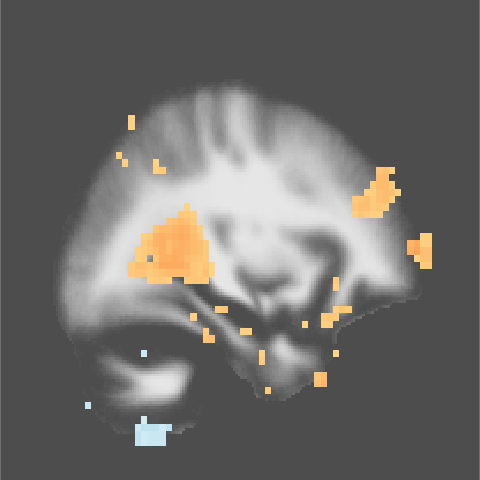
\includegraphics[width=0.16\linewidth]{cor-sagital-age-t-mW} &
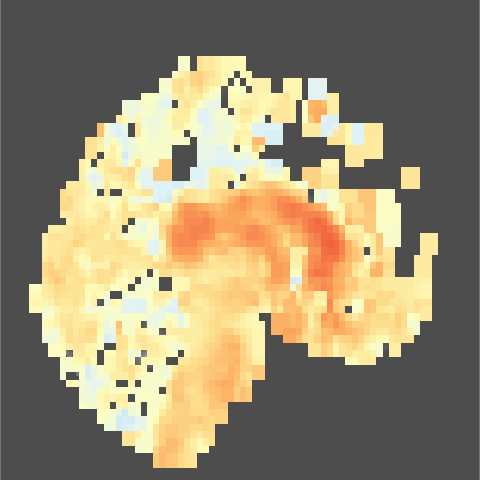
\includegraphics[width=0.16\linewidth]{cor-sagital-cdr-mW} &
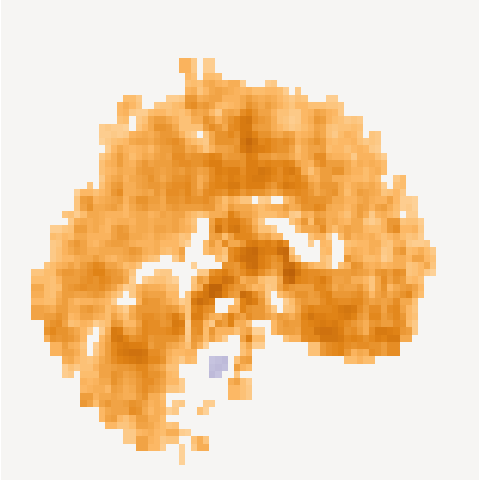
\includegraphics[width=0.16\linewidth]{cor-sagital-cdr-t-mW} &
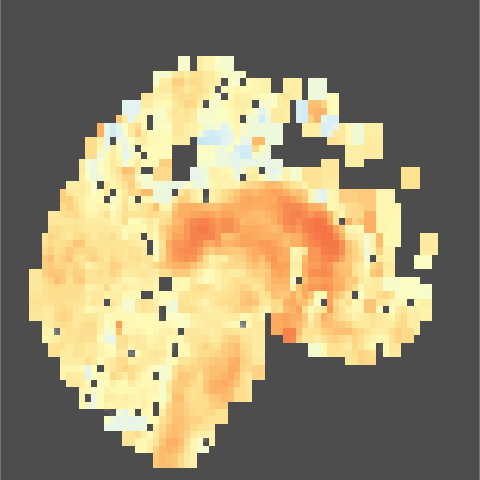
\includegraphics[width=0.16\linewidth]{cor-sagital-mmse-mW} &
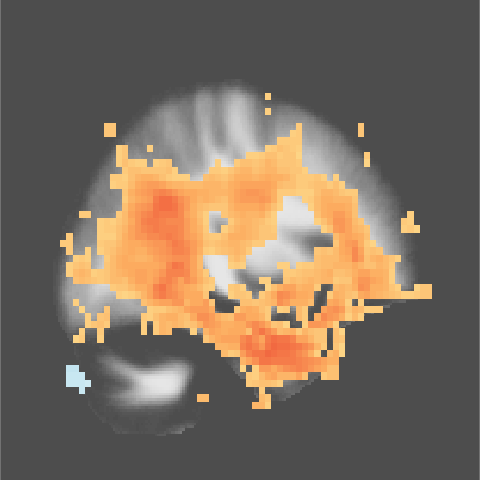
\includegraphics[width=0.16\linewidth]{cor-sagital-mmse-t-mW} \\ \hline \hline
%
\parbox[t]{2mm}{\multirow{3}{*}{\rotatebox[origin=c]{90}{Transport Cost}}}&
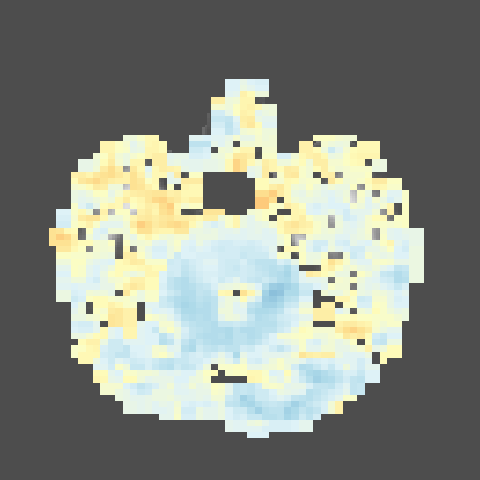
\includegraphics[width=0.16\linewidth]{cor-axial-age-tW} &
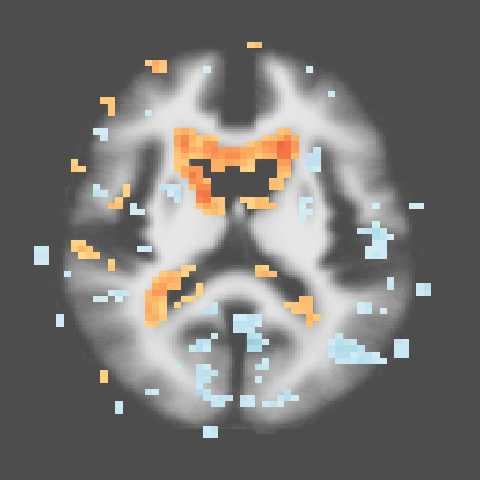
\includegraphics[width=0.16\linewidth]{cor-axial-age-t-tW} &
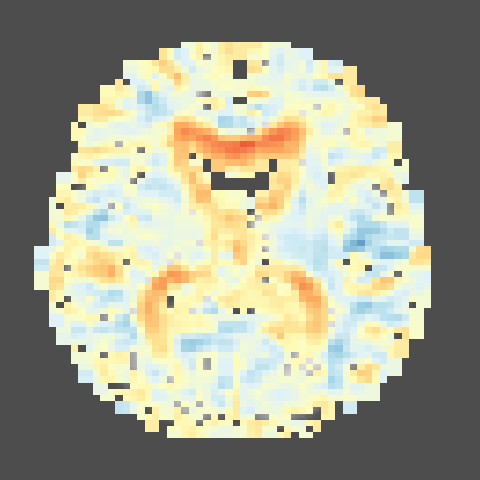
\includegraphics[width=0.16\linewidth]{cor-axial-cdr-tW} &
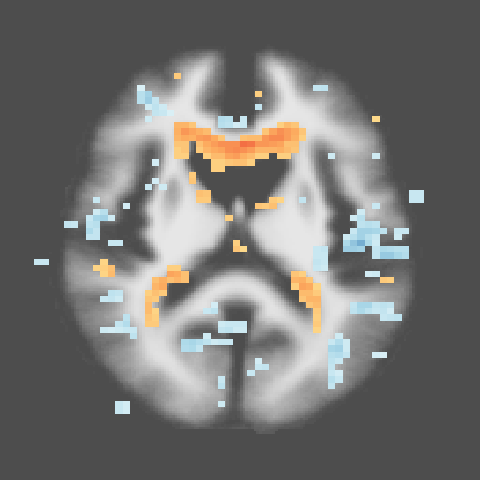
\includegraphics[width=0.16\linewidth]{cor-axial-cdr-t-tW} &
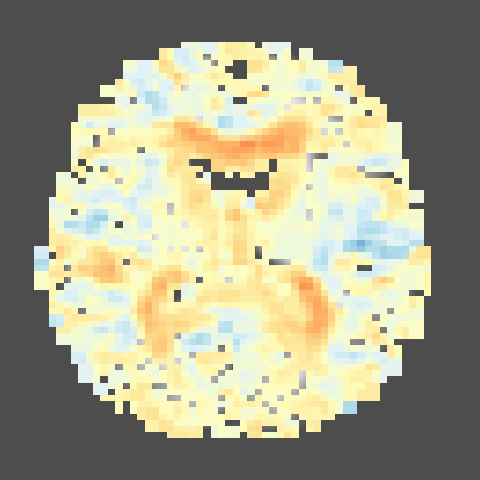
\includegraphics[width=0.16\linewidth]{cor-axial-mmse-tW} &
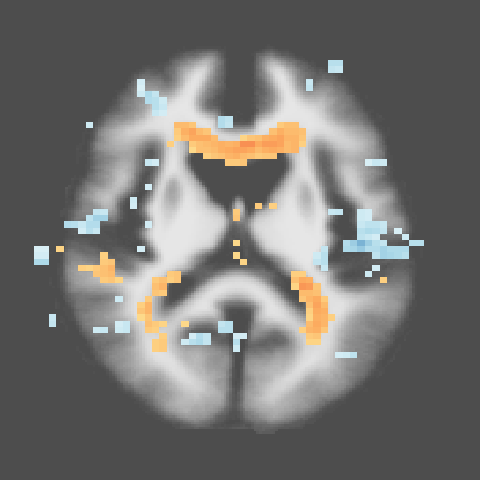
\includegraphics[width=0.16\linewidth]{cor-axial-mmse-t-tW} \\ 
%
        &
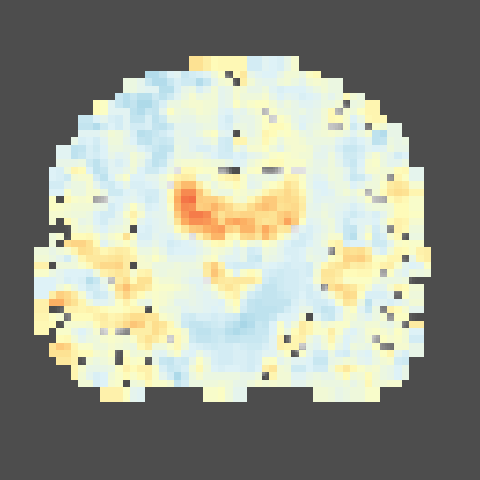
\includegraphics[width=0.16\linewidth]{cor-coronal-age-tW} &
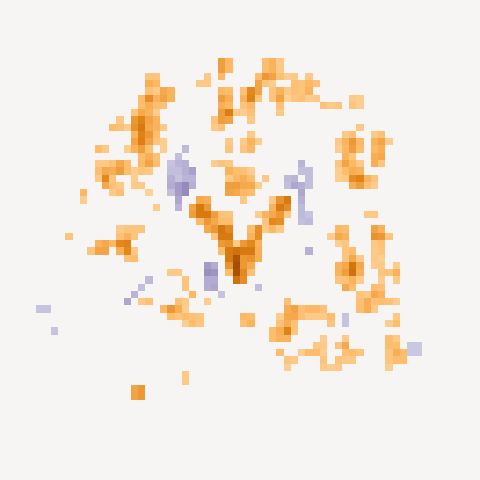
\includegraphics[width=0.16\linewidth]{cor-coronal-age-t-tW} &
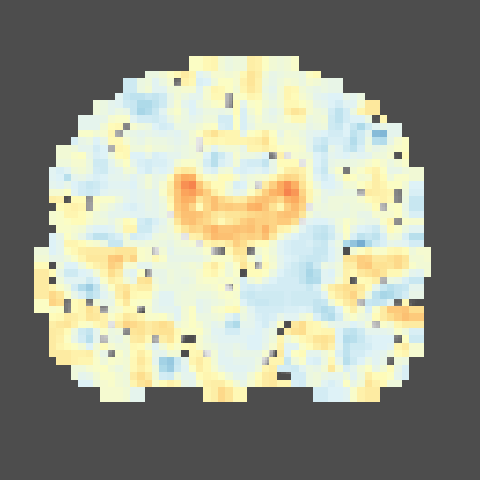
\includegraphics[width=0.16\linewidth]{cor-coronal-cdr-tW} &
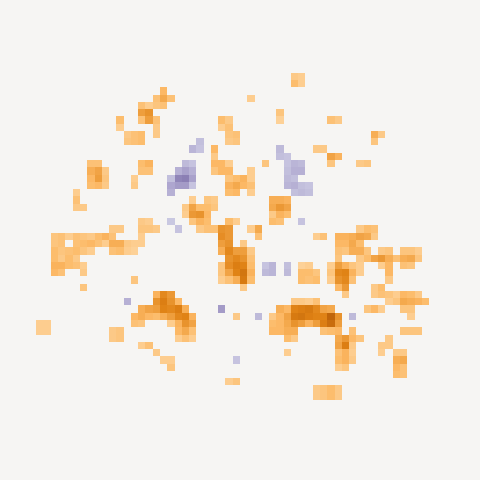
\includegraphics[width=0.16\linewidth]{cor-coronal-cdr-t-tW} &
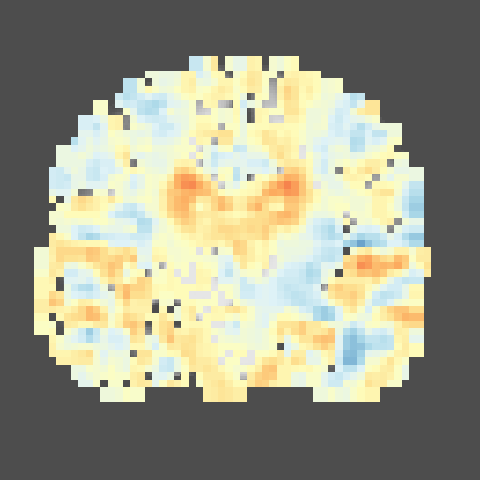
\includegraphics[width=0.16\linewidth]{cor-coronal-mmse-tW} &
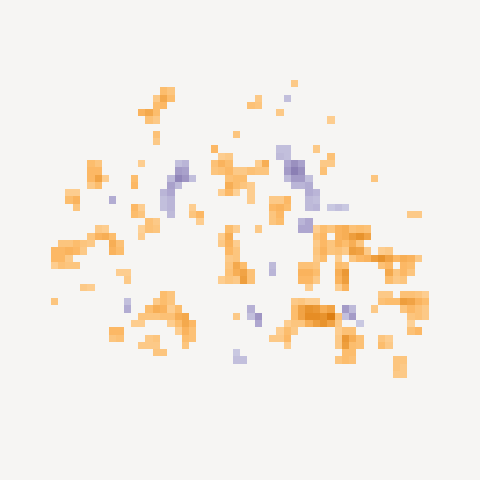
\includegraphics[width=0.16\linewidth]{cor-coronal-mmse-t-tW} \\ 
%
        &
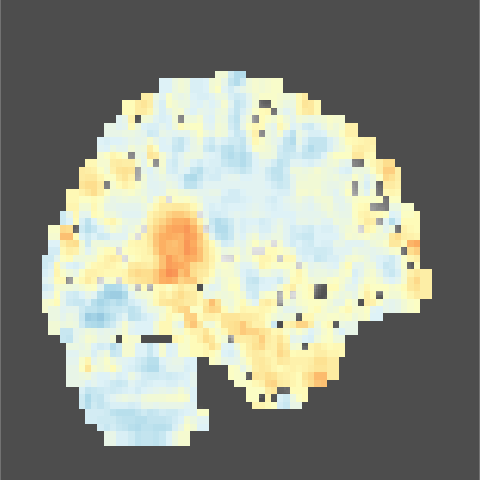
\includegraphics[width=0.16\linewidth]{cor-sagital-age-tW} &
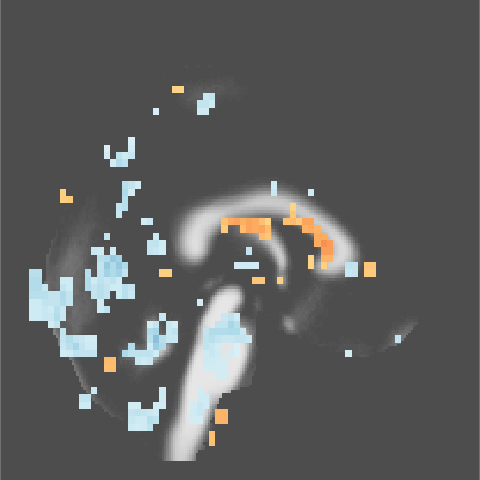
\includegraphics[width=0.16\linewidth]{cor-sagital-age-t-tW} &
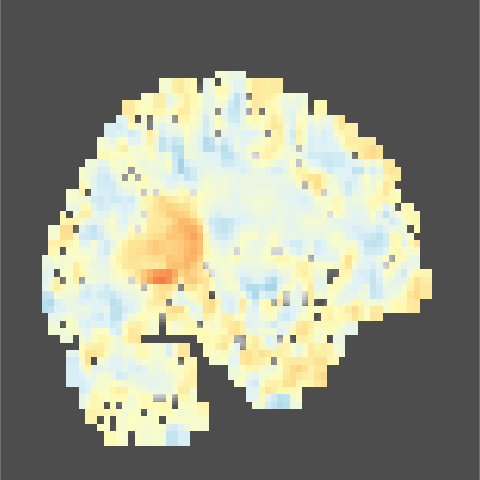
\includegraphics[width=0.16\linewidth]{cor-sagital-cdr-tW} &
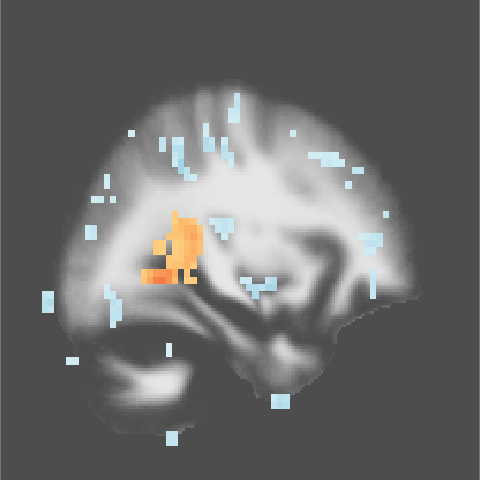
\includegraphics[width=0.16\linewidth]{cor-sagital-cdr-t-tW} &
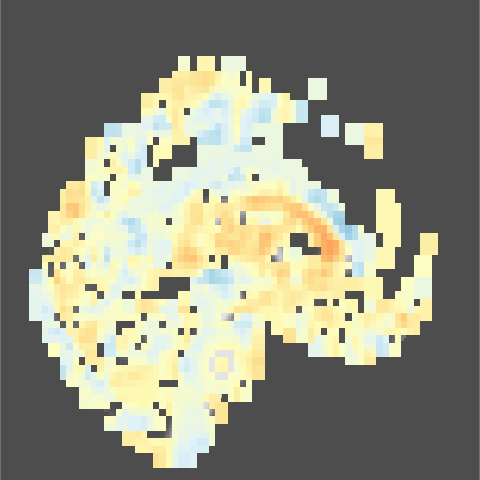
\includegraphics[width=0.16\linewidth]{cor-sagital-mmse-tW} &
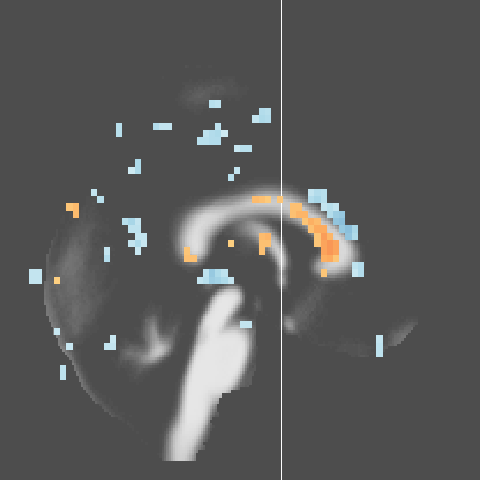
\includegraphics[width=0.16\linewidth]{cor-sagital-mmse-t-tW} \\ \hline \hline
%
& \parbox[b][4mm]{6mm}{Age} 
& \parbox[b][4mm]{6mm}{Age\textsuperscript{*}} 
& \parbox[b][4mm]{6mm}{CDR} 
& \parbox[b][4mm]{6mm}{CDR\textsuperscript{*}}
& \parbox[b][4mm]{6mm}{MMSE}
& \parbox[b][4mm]{6mm}{MMSE\textsuperscript{*}}
\end{tabular}
\caption{\label{fig:cor-oasis-gray}
Correlation of age, MMSE and CDR with optimal transport mass imbalances and
optimal transport costs of gray matter. The columns with a \textsuperscript{*}
only show the voxels were the correlation has a permutation tested p-value less
than 0.05  }
\end{figure}
\endgroup

\begingroup
\renewcommand{\arraystretch}{0}
\setlength{\tabcolsep}{0pt}
\begin{figure}[bth]
\centering
\begin{tabular}{l|cc|cc|cc}
\parbox[t]{4mm}{\multirow{3}{*}{\rotatebox[origin=c]{90}{Mass Imbalance}}}&
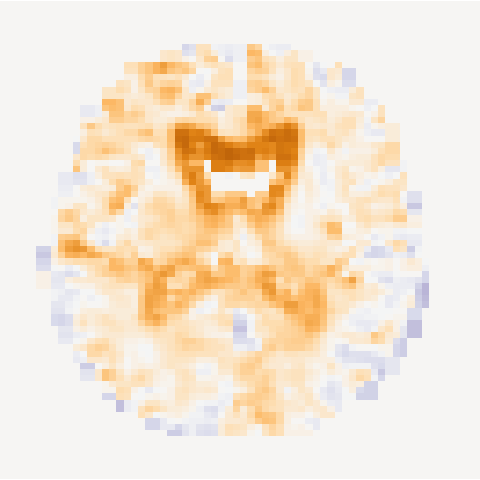
\includegraphics[width=0.16\linewidth]{cor-axial-age-mG} &
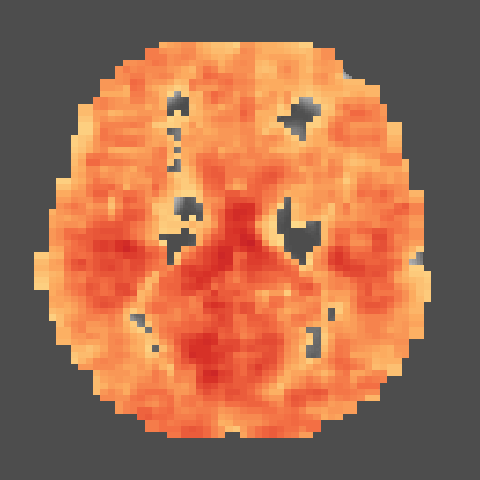
\includegraphics[width=0.16\linewidth]{cor-axial-age-t-mG} &
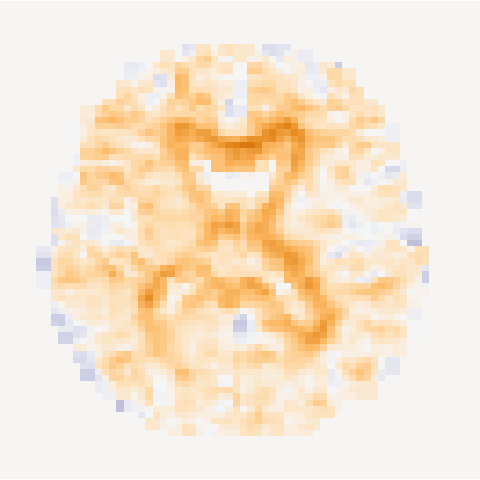
\includegraphics[width=0.16\linewidth]{cor-axial-cdr-mG} &
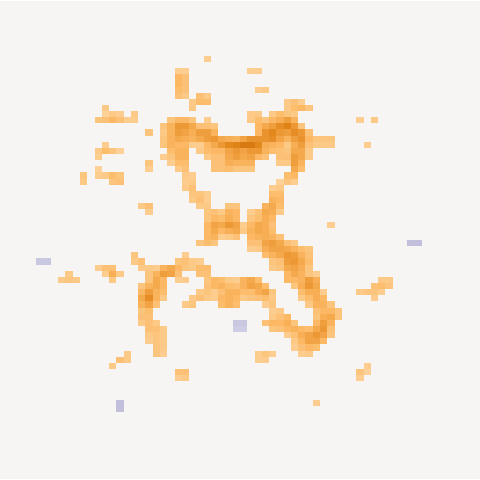
\includegraphics[width=0.16\linewidth]{cor-axial-cdr-t-mG} &
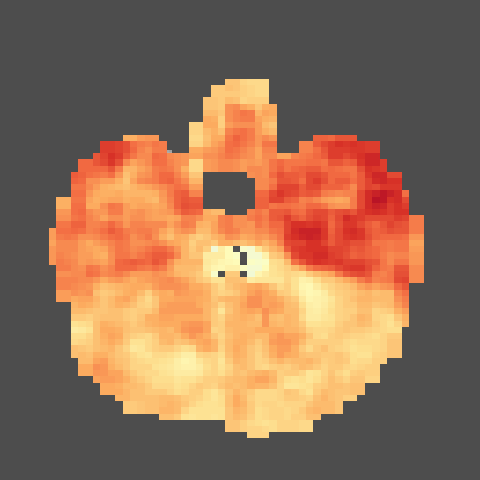
\includegraphics[width=0.16\linewidth]{cor-axial-mmse-mG} &
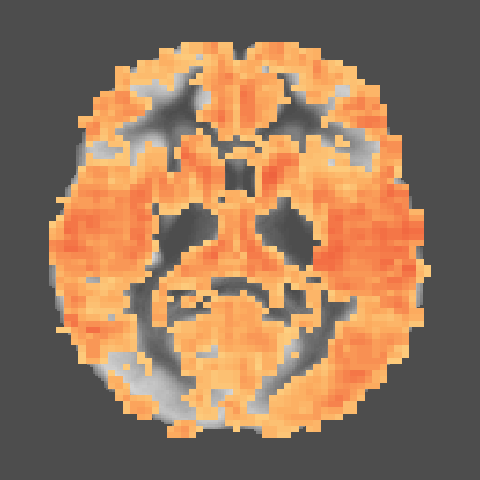
\includegraphics[width=0.16\linewidth]{cor-axial-mmse-t-mG} \\ 
%
        &
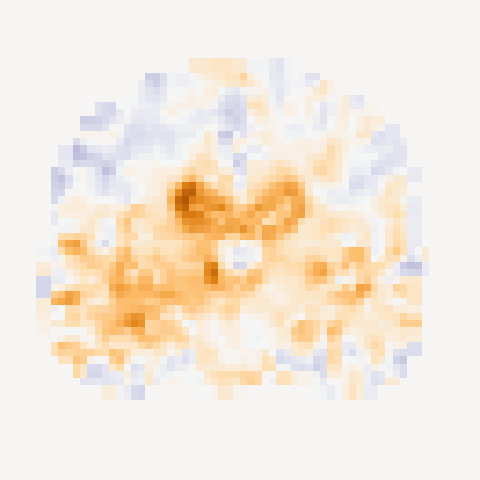
\includegraphics[width=0.16\linewidth]{cor-coronal-age-mG} &
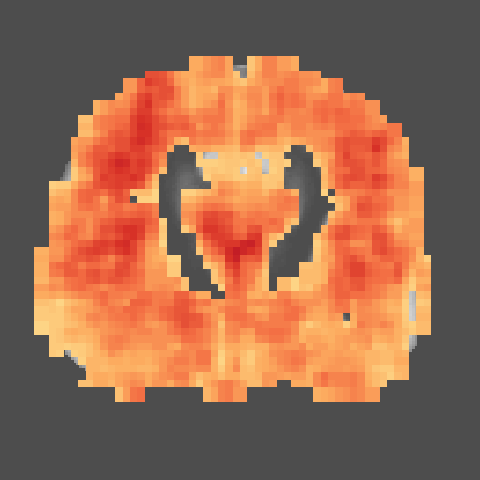
\includegraphics[width=0.16\linewidth]{cor-coronal-age-t-mG} &
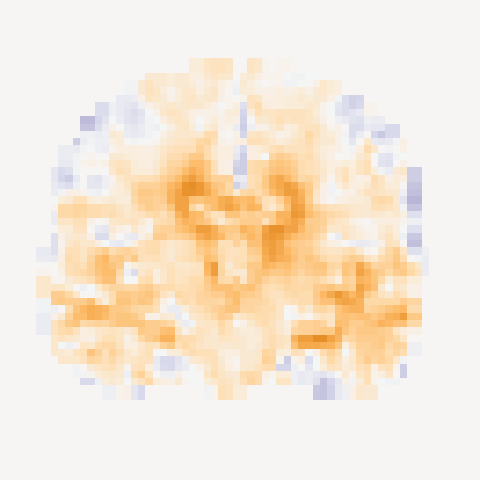
\includegraphics[width=0.16\linewidth]{cor-coronal-cdr-mG} &

\includegraphics[width=0.16\linewidth]{cor-coronal-cdr-t-mG} &
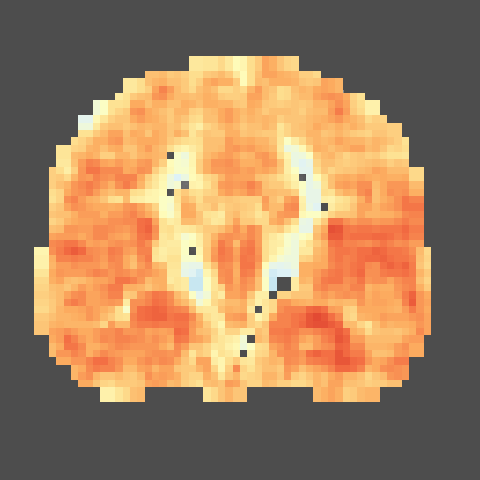
\includegraphics[width=0.16\linewidth]{cor-coronal-mmse-mG} &
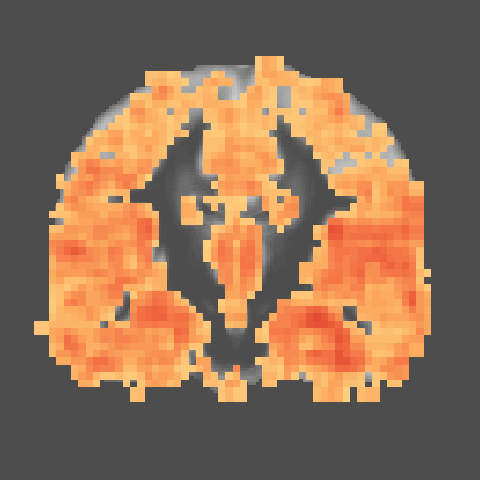
\includegraphics[width=0.16\linewidth]{cor-coronal-mmse-t-mG} \\ 
%
        &
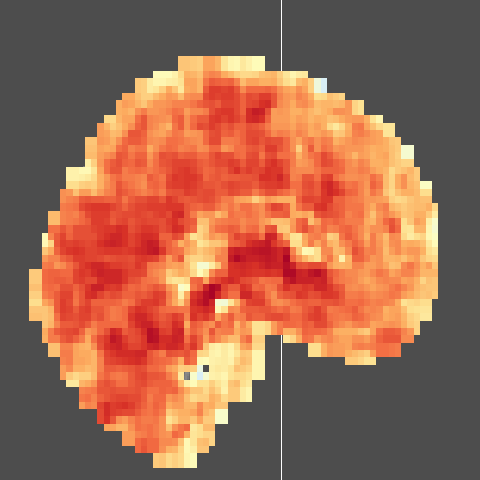
\includegraphics[width=0.16\linewidth]{cor-sagital-age-mG} &
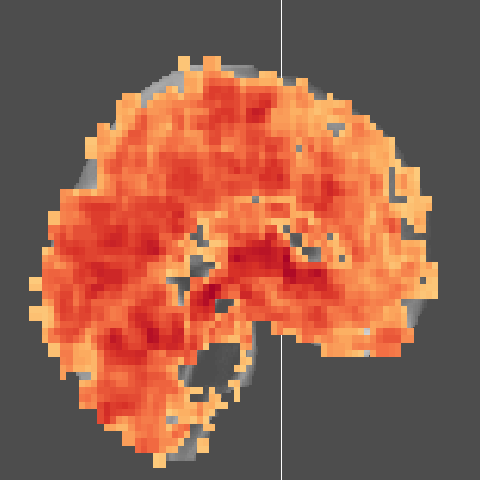
\includegraphics[width=0.16\linewidth]{cor-sagital-age-t-mG} &
\includegraphics[width=0.16\linewidth]{cor-sagital-cdr-mG} &
\includegraphics[width=0.16\linewidth]{cor-sagital-cdr-t-mG} &
\includegraphics[width=0.16\linewidth]{cor-sagital-mmse-mG} &
\includegraphics[width=0.16\linewidth]{cor-sagital-mmse-t-mG} \\ \hline \hline
%
\parbox[t]{2mm}{\multirow{3}{*}{\rotatebox[origin=c]{90}{Transport Cost}}}&
\includegraphics[width=0.16\linewidth]{cor-axial-age-tG} &
\includegraphics[width=0.16\linewidth]{cor-axial-age-t-tG} &
\includegraphics[width=0.16\linewidth]{cor-axial-cdr-tG} &
\includegraphics[width=0.16\linewidth]{cor-axial-cdr-t-tG} &
\includegraphics[width=0.16\linewidth]{cor-axial-mmse-tG} &
\includegraphics[width=0.16\linewidth]{cor-axial-mmse-t-tG} \\ 
%
        &
\includegraphics[width=0.16\linewidth]{cor-coronal-age-tG} &
\includegraphics[width=0.16\linewidth]{cor-coronal-age-t-tG} &
\includegraphics[width=0.16\linewidth]{cor-coronal-cdr-tG} &
\includegraphics[width=0.16\linewidth]{cor-coronal-cdr-t-tG} &
\includegraphics[width=0.16\linewidth]{cor-coronal-mmse-tG} &
\includegraphics[width=0.16\linewidth]{cor-coronal-mmse-t-tG} \\ 
%
        &
\includegraphics[width=0.16\linewidth]{cor-sagital-age-tG} &
\includegraphics[width=0.16\linewidth]{cor-sagital-age-t-tG} &
\includegraphics[width=0.16\linewidth]{cor-sagital-cdr-tG} &
\includegraphics[width=0.16\linewidth]{cor-sagital-cdr-t-tG} &
\includegraphics[width=0.16\linewidth]{cor-sagital-mmse-tG} &
\includegraphics[width=0.16\linewidth]{cor-sagital-mmse-t-tG} \\ \hline \hline
%%
& \parbox[b][4mm]{6mm}{Age} 
& \parbox[b][4mm]{6mm}{Age\textsuperscript{*}} 
& \parbox[b][4mm]{6mm}{CDR} 
& \parbox[b][4mm]{6mm}{CDR\textsuperscript{*}}
& \parbox[b][4mm]{6mm}{MMSE}
& \parbox[b][4mm]{6mm}{MMSE\textsuperscript{*}}
\end{tabular}
\caption{\label{fig:cor-oasis-white}
Correlation of age, MMSE and CDR with optimal transport mass imbalances and
optimal transport costs of white matter. The columns with a \textsuperscript{*}
only show the voxels were the correlation has a permutation tested p-value less
than 0.05  }
\end{figure}
\endgroup



